% Options for packages loaded elsewhere
\PassOptionsToPackage{unicode}{hyperref}
\PassOptionsToPackage{hyphens}{url}
%
\documentclass[
]{article}
\usepackage{amsmath,amssymb}
\usepackage{lmodern}
\usepackage{iftex}
\ifPDFTeX
  \usepackage[T1]{fontenc}
  \usepackage[utf8]{inputenc}
  \usepackage{textcomp} % provide euro and other symbols
\else % if luatex or xetex
  \usepackage{unicode-math}
  \defaultfontfeatures{Scale=MatchLowercase}
  \defaultfontfeatures[\rmfamily]{Ligatures=TeX,Scale=1}
\fi
% Use upquote if available, for straight quotes in verbatim environments
\IfFileExists{upquote.sty}{\usepackage{upquote}}{}
\IfFileExists{microtype.sty}{% use microtype if available
  \usepackage[]{microtype}
  \UseMicrotypeSet[protrusion]{basicmath} % disable protrusion for tt fonts
}{}
\makeatletter
\@ifundefined{KOMAClassName}{% if non-KOMA class
  \IfFileExists{parskip.sty}{%
    \usepackage{parskip}
  }{% else
    \setlength{\parindent}{0pt}
    \setlength{\parskip}{6pt plus 2pt minus 1pt}}
}{% if KOMA class
  \KOMAoptions{parskip=half}}
\makeatother
\usepackage{xcolor}
\usepackage[margin=1in]{geometry}
\usepackage{color}
\usepackage{fancyvrb}
\newcommand{\VerbBar}{|}
\newcommand{\VERB}{\Verb[commandchars=\\\{\}]}
\DefineVerbatimEnvironment{Highlighting}{Verbatim}{commandchars=\\\{\}}
% Add ',fontsize=\small' for more characters per line
\usepackage{framed}
\definecolor{shadecolor}{RGB}{248,248,248}
\newenvironment{Shaded}{\begin{snugshade}}{\end{snugshade}}
\newcommand{\AlertTok}[1]{\textcolor[rgb]{0.94,0.16,0.16}{#1}}
\newcommand{\AnnotationTok}[1]{\textcolor[rgb]{0.56,0.35,0.01}{\textbf{\textit{#1}}}}
\newcommand{\AttributeTok}[1]{\textcolor[rgb]{0.77,0.63,0.00}{#1}}
\newcommand{\BaseNTok}[1]{\textcolor[rgb]{0.00,0.00,0.81}{#1}}
\newcommand{\BuiltInTok}[1]{#1}
\newcommand{\CharTok}[1]{\textcolor[rgb]{0.31,0.60,0.02}{#1}}
\newcommand{\CommentTok}[1]{\textcolor[rgb]{0.56,0.35,0.01}{\textit{#1}}}
\newcommand{\CommentVarTok}[1]{\textcolor[rgb]{0.56,0.35,0.01}{\textbf{\textit{#1}}}}
\newcommand{\ConstantTok}[1]{\textcolor[rgb]{0.00,0.00,0.00}{#1}}
\newcommand{\ControlFlowTok}[1]{\textcolor[rgb]{0.13,0.29,0.53}{\textbf{#1}}}
\newcommand{\DataTypeTok}[1]{\textcolor[rgb]{0.13,0.29,0.53}{#1}}
\newcommand{\DecValTok}[1]{\textcolor[rgb]{0.00,0.00,0.81}{#1}}
\newcommand{\DocumentationTok}[1]{\textcolor[rgb]{0.56,0.35,0.01}{\textbf{\textit{#1}}}}
\newcommand{\ErrorTok}[1]{\textcolor[rgb]{0.64,0.00,0.00}{\textbf{#1}}}
\newcommand{\ExtensionTok}[1]{#1}
\newcommand{\FloatTok}[1]{\textcolor[rgb]{0.00,0.00,0.81}{#1}}
\newcommand{\FunctionTok}[1]{\textcolor[rgb]{0.00,0.00,0.00}{#1}}
\newcommand{\ImportTok}[1]{#1}
\newcommand{\InformationTok}[1]{\textcolor[rgb]{0.56,0.35,0.01}{\textbf{\textit{#1}}}}
\newcommand{\KeywordTok}[1]{\textcolor[rgb]{0.13,0.29,0.53}{\textbf{#1}}}
\newcommand{\NormalTok}[1]{#1}
\newcommand{\OperatorTok}[1]{\textcolor[rgb]{0.81,0.36,0.00}{\textbf{#1}}}
\newcommand{\OtherTok}[1]{\textcolor[rgb]{0.56,0.35,0.01}{#1}}
\newcommand{\PreprocessorTok}[1]{\textcolor[rgb]{0.56,0.35,0.01}{\textit{#1}}}
\newcommand{\RegionMarkerTok}[1]{#1}
\newcommand{\SpecialCharTok}[1]{\textcolor[rgb]{0.00,0.00,0.00}{#1}}
\newcommand{\SpecialStringTok}[1]{\textcolor[rgb]{0.31,0.60,0.02}{#1}}
\newcommand{\StringTok}[1]{\textcolor[rgb]{0.31,0.60,0.02}{#1}}
\newcommand{\VariableTok}[1]{\textcolor[rgb]{0.00,0.00,0.00}{#1}}
\newcommand{\VerbatimStringTok}[1]{\textcolor[rgb]{0.31,0.60,0.02}{#1}}
\newcommand{\WarningTok}[1]{\textcolor[rgb]{0.56,0.35,0.01}{\textbf{\textit{#1}}}}
\usepackage{longtable,booktabs,array}
\usepackage{calc} % for calculating minipage widths
% Correct order of tables after \paragraph or \subparagraph
\usepackage{etoolbox}
\makeatletter
\patchcmd\longtable{\par}{\if@noskipsec\mbox{}\fi\par}{}{}
\makeatother
% Allow footnotes in longtable head/foot
\IfFileExists{footnotehyper.sty}{\usepackage{footnotehyper}}{\usepackage{footnote}}
\makesavenoteenv{longtable}
\usepackage{graphicx}
\makeatletter
\def\maxwidth{\ifdim\Gin@nat@width>\linewidth\linewidth\else\Gin@nat@width\fi}
\def\maxheight{\ifdim\Gin@nat@height>\textheight\textheight\else\Gin@nat@height\fi}
\makeatother
% Scale images if necessary, so that they will not overflow the page
% margins by default, and it is still possible to overwrite the defaults
% using explicit options in \includegraphics[width, height, ...]{}
\setkeys{Gin}{width=\maxwidth,height=\maxheight,keepaspectratio}
% Set default figure placement to htbp
\makeatletter
\def\fps@figure{htbp}
\makeatother
\setlength{\emergencystretch}{3em} % prevent overfull lines
\providecommand{\tightlist}{%
  \setlength{\itemsep}{0pt}\setlength{\parskip}{0pt}}
\setcounter{secnumdepth}{-\maxdimen} % remove section numbering
\ifLuaTeX
  \usepackage{selnolig}  % disable illegal ligatures
\fi
\IfFileExists{bookmark.sty}{\usepackage{bookmark}}{\usepackage{hyperref}}
\IfFileExists{xurl.sty}{\usepackage{xurl}}{} % add URL line breaks if available
\urlstyle{same} % disable monospaced font for URLs
\hypersetup{
  pdftitle={Genetic differentiation on flowering time in Cerastium fontanum using a greenhouse experiment},
  pdfauthor={Alicia Valdés},
  hidelinks,
  pdfcreator={LaTeX via pandoc}}

\title{Genetic differentiation on flowering time in Cerastium fontanum
using a greenhouse experiment}
\usepackage{etoolbox}
\makeatletter
\providecommand{\subtitle}[1]{% add subtitle to \maketitle
  \apptocmd{\@title}{\par {\large #1 \par}}{}{}
}
\makeatother
\subtitle{Data preparation and first analyses}
\author{Alicia Valdés}
\date{07 mars, 2023}

\begin{document}
\maketitle

{
\setcounter{tocdepth}{4}
\tableofcontents
}
\hypertarget{data-preparation}{%
\section{Data preparation}\label{data-preparation}}

\hypertarget{read-data-from-excel-files}{%
\subsection{Read data from Excel
files}\label{read-data-from-excel-files}}

\begin{Shaded}
\begin{Highlighting}[]
\NormalTok{data\_exp}\OtherTok{\textless{}{-}}\FunctionTok{read\_excel}\NormalTok{(}\StringTok{"data/edited/Cerastium\_greenhouse\_spring\_2022.xlsx"}\NormalTok{, }
                       \AttributeTok{sheet=}\StringTok{"extracted\_data"}\NormalTok{)}
\NormalTok{data\_exp}\SpecialCharTok{$}\NormalTok{treat}\OtherTok{\textless{}{-}}\FunctionTok{as.factor}\NormalTok{(data\_exp}\SpecialCharTok{$}\NormalTok{treat)}
\NormalTok{data\_exp}\SpecialCharTok{$}\NormalTok{mother}\OtherTok{\textless{}{-}}\FunctionTok{as.factor}\NormalTok{(data\_exp}\SpecialCharTok{$}\NormalTok{mother)}
\NormalTok{data\_exp}\SpecialCharTok{$}\NormalTok{father}\OtherTok{\textless{}{-}}\FunctionTok{as.factor}\NormalTok{(data\_exp}\SpecialCharTok{$}\NormalTok{father)}
\NormalTok{data\_exp}\SpecialCharTok{$}\NormalTok{total\_n\_fl}\OtherTok{\textless{}{-}}\FunctionTok{as.integer}\NormalTok{(data\_exp}\SpecialCharTok{$}\NormalTok{total\_n\_fl)}
\NormalTok{data\_exp}\SpecialCharTok{$}\NormalTok{date50}\OtherTok{\textless{}{-}}\FunctionTok{as.numeric}\NormalTok{(data\_exp}\SpecialCharTok{$}\NormalTok{date50)}
\end{Highlighting}
\end{Shaded}

\begin{Shaded}
\begin{Highlighting}[]
\NormalTok{data\_parents}\OtherTok{\textless{}{-}}\FunctionTok{read\_excel}\NormalTok{(}\StringTok{"data/edited/Cerastium\_greenhouse\_spring\_2022.xlsx"}\NormalTok{, }
                       \AttributeTok{sheet=}\StringTok{"extracted\_data\_parents"}\NormalTok{)}
\NormalTok{data\_parents}\SpecialCharTok{$}\NormalTok{treat}\OtherTok{\textless{}{-}}\FunctionTok{as.factor}\NormalTok{(data\_parents}\SpecialCharTok{$}\NormalTok{treat)}
\end{Highlighting}
\end{Shaded}

\begin{Shaded}
\begin{Highlighting}[]
\FunctionTok{head}\NormalTok{(data\_exp)}
\end{Highlighting}
\end{Shaded}

\begin{verbatim}
## # A tibble: 6 x 10
##   mother father temp_mother temp_father treat    total_n_fl   FFD   LFD date50
##   <fct>  <fct>        <dbl>       <dbl> <fct>         <int> <dbl> <dbl>  <dbl>
## 1 16     120           25.9        11.3 unheated         13   129   154    138
## 2 39     350           22.6        20.6 unheated          0    NA    NA     NA
## 3 26     250           21.5        23.4 unheated          6   124   140    129
## 4 31     310            7           8   unheated         64   115   150    128
## 5 24     210           14.9         7   unheated          6   124   145    129
## 6 34     320           18           9   unheated         15   129   161    138
##   Comments
##   <chr>   
## 1 <NA>    
## 2 <NA>    
## 3 <NA>    
## 4 <NA>    
## 5 <NA>    
## 6 <NA>
\end{verbatim}

\begin{Shaded}
\begin{Highlighting}[]
\FunctionTok{head}\NormalTok{(data\_parents)}
\end{Highlighting}
\end{Shaded}

\begin{verbatim}
## # A tibble: 6 x 8
##   id_parent  temp treat    total_n_fl   FFD   LFD date50 Comments              
##       <dbl> <dbl> <fct>         <dbl> <dbl> <dbl>  <dbl> <chr>                 
## 1        13  12   unheated         13   129   152    139 <NA>                  
## 2        13  12   heatmat          16   124   131    125 <NA>                  
## 3        13  12   heatmat           4   126   136    131 <NA>                  
## 4        14  29.8 unheated          2   133   136    133 Both mother and father
## 5        14  29.8 heatmat           1   138   138    137 Both mother and father
## 6        14  29.8 heatmat           2   131   136    131 Both mother and father
\end{verbatim}

\hypertarget{how-many-different-mothers-and-fathers}{%
\subsection{How many different mothers and
fathers?}\label{how-many-different-mothers-and-fathers}}

\begin{Shaded}
\begin{Highlighting}[]
\FunctionTok{length}\NormalTok{(}\FunctionTok{levels}\NormalTok{(data\_exp}\SpecialCharTok{$}\NormalTok{mother)) }\CommentTok{\# 25 different mothers (shouldn\textquotesingle{}t it be 24?)}
\end{Highlighting}
\end{Shaded}

\begin{verbatim}
## [1] 25
\end{verbatim}

\begin{Shaded}
\begin{Highlighting}[]
\FunctionTok{length}\NormalTok{(}\FunctionTok{levels}\NormalTok{(data\_exp}\SpecialCharTok{$}\NormalTok{father)) }\CommentTok{\# 24 different mothers}
\end{Highlighting}
\end{Shaded}

\begin{verbatim}
## [1] 24
\end{verbatim}

\hypertarget{how-many-unique-combinations-of-mothers-and-fathers}{%
\subsection{How many unique combinations of mothers and
fathers?}\label{how-many-unique-combinations-of-mothers-and-fathers}}

\begin{Shaded}
\begin{Highlighting}[]
\NormalTok{data\_exp}\OtherTok{\textless{}{-}}\NormalTok{data\_exp}\SpecialCharTok{\%\textgreater{}\%}\FunctionTok{mutate}\NormalTok{(}\AttributeTok{mother\_father=}\FunctionTok{paste}\NormalTok{(mother,father,}\AttributeTok{sep=}\StringTok{"\_"}\NormalTok{))}
\end{Highlighting}
\end{Shaded}

\begin{Shaded}
\begin{Highlighting}[]
\FunctionTok{length}\NormalTok{(}\FunctionTok{unique}\NormalTok{(data\_exp}\SpecialCharTok{$}\NormalTok{mother\_father)) }\CommentTok{\# 100 (shouldn\textquotesingle{}t it be 96?)}
\end{Highlighting}
\end{Shaded}

\begin{verbatim}
## [1] 100
\end{verbatim}

\begin{Shaded}
\begin{Highlighting}[]
\CommentTok{\# It is really 99, because one is "NA\_NA"}
\end{Highlighting}
\end{Shaded}

\hypertarget{number-of-plants-from-each-crossing}{%
\subsection{Number of plants from each
crossing}\label{number-of-plants-from-each-crossing}}

\begin{Shaded}
\begin{Highlighting}[]
\NormalTok{data\_exp}\SpecialCharTok{\%\textgreater{}\%}\FunctionTok{group\_by}\NormalTok{(mother\_father)}\SpecialCharTok{\%\textgreater{}\%}\FunctionTok{summarise}\NormalTok{(}\AttributeTok{num=}\FunctionTok{n}\NormalTok{())}\SpecialCharTok{\%\textgreater{}\%}
  \FunctionTok{ggplot}\NormalTok{(}\FunctionTok{aes}\NormalTok{(}\AttributeTok{x=}\NormalTok{num))}\SpecialCharTok{+}\FunctionTok{geom\_histogram}\NormalTok{(}\AttributeTok{bins=}\DecValTok{12}\NormalTok{)}
\end{Highlighting}
\end{Shaded}

\includegraphics{1_data_prep_analyses_files/figure-latex/unnamed-chunk-7-1.pdf}

12 plants from most crossings, but also one with 13 and some with fewer.

\hypertarget{distributions}{%
\section{Distributions}\label{distributions}}

\begin{Shaded}
\begin{Highlighting}[]
\FunctionTok{hist}\NormalTok{(data\_exp}\SpecialCharTok{$}\NormalTok{FFD)}
\end{Highlighting}
\end{Shaded}

\includegraphics{1_data_prep_analyses_files/figure-latex/unnamed-chunk-8-1.pdf}

\begin{Shaded}
\begin{Highlighting}[]
\FunctionTok{hist}\NormalTok{(data\_exp}\SpecialCharTok{$}\NormalTok{LFD)}
\end{Highlighting}
\end{Shaded}

\includegraphics{1_data_prep_analyses_files/figure-latex/unnamed-chunk-8-2.pdf}

\begin{Shaded}
\begin{Highlighting}[]
\FunctionTok{hist}\NormalTok{(data\_exp}\SpecialCharTok{$}\NormalTok{date50)}
\end{Highlighting}
\end{Shaded}

\includegraphics{1_data_prep_analyses_files/figure-latex/unnamed-chunk-8-3.pdf}

All looking quite normal.

\hypertarget{analyses}{%
\section{Analyses}\label{analyses}}

\hypertarget{with-offspring-from-crosses}{%
\subsection{With offspring from
crosses}\label{with-offspring-from-crosses}}

Including mother, father and crossing as random factors.

\begin{Shaded}
\begin{Highlighting}[]
\NormalTok{model\_offpsring\_FFD}\OtherTok{\textless{}{-}}\FunctionTok{glmmTMB}\NormalTok{(FFD}\SpecialCharTok{\textasciitilde{}}\NormalTok{(temp\_mother}\SpecialCharTok{+}\NormalTok{temp\_father)}\SpecialCharTok{*}\NormalTok{treat}\SpecialCharTok{+}
\NormalTok{                               (}\DecValTok{1}\SpecialCharTok{|}\NormalTok{mother)}\SpecialCharTok{+}\NormalTok{(}\DecValTok{1}\SpecialCharTok{|}\NormalTok{father)}\SpecialCharTok{+}\NormalTok{(}\DecValTok{1}\SpecialCharTok{|}\NormalTok{mother\_father),data\_exp)}
\NormalTok{model\_offpsring\_LFD}\OtherTok{\textless{}{-}}\FunctionTok{glmmTMB}\NormalTok{(LFD}\SpecialCharTok{\textasciitilde{}}\NormalTok{(temp\_mother}\SpecialCharTok{+}\NormalTok{temp\_father)}\SpecialCharTok{*}\NormalTok{treat}\SpecialCharTok{+}
\NormalTok{                               (}\DecValTok{1}\SpecialCharTok{|}\NormalTok{mother)}\SpecialCharTok{+}\NormalTok{(}\DecValTok{1}\SpecialCharTok{|}\NormalTok{father)}\SpecialCharTok{+}\NormalTok{(}\DecValTok{1}\SpecialCharTok{|}\NormalTok{mother\_father),data\_exp)}
\NormalTok{model\_offpsring\_date50}\OtherTok{\textless{}{-}}\FunctionTok{glmmTMB}\NormalTok{(date50}\SpecialCharTok{\textasciitilde{}}\NormalTok{(temp\_mother}\SpecialCharTok{+}\NormalTok{temp\_father)}\SpecialCharTok{*}\NormalTok{treat}\SpecialCharTok{+}
\NormalTok{                               (}\DecValTok{1}\SpecialCharTok{|}\NormalTok{mother)}\SpecialCharTok{+}\NormalTok{(}\DecValTok{1}\SpecialCharTok{|}\NormalTok{father)}\SpecialCharTok{+}\NormalTok{(}\DecValTok{1}\SpecialCharTok{|}\NormalTok{mother\_father),data\_exp)}
\end{Highlighting}
\end{Shaded}

\begin{Shaded}
\begin{Highlighting}[]
\FunctionTok{kable}\NormalTok{(}\FunctionTok{tidy}\NormalTok{(model\_offpsring\_FFD),}\AttributeTok{digits=}\FunctionTok{c}\NormalTok{(}\DecValTok{3}\NormalTok{,}\DecValTok{3}\NormalTok{,}\DecValTok{2}\NormalTok{,}\DecValTok{3}\NormalTok{))}
\end{Highlighting}
\end{Shaded}

\begin{longtable}[]{@{}
  >{\raggedright\arraybackslash}p{(\columnwidth - 14\tabcolsep) * \real{0.0938}}
  >{\raggedright\arraybackslash}p{(\columnwidth - 14\tabcolsep) * \real{0.1042}}
  >{\raggedright\arraybackslash}p{(\columnwidth - 14\tabcolsep) * \real{0.1458}}
  >{\raggedright\arraybackslash}p{(\columnwidth - 14\tabcolsep) * \real{0.2708}}
  >{\raggedleft\arraybackslash}p{(\columnwidth - 14\tabcolsep) * \real{0.0938}}
  >{\raggedleft\arraybackslash}p{(\columnwidth - 14\tabcolsep) * \real{0.1042}}
  >{\raggedleft\arraybackslash}p{(\columnwidth - 14\tabcolsep) * \real{0.1042}}
  >{\raggedleft\arraybackslash}p{(\columnwidth - 14\tabcolsep) * \real{0.0833}}@{}}
\toprule()
\begin{minipage}[b]{\linewidth}\raggedright
effect
\end{minipage} & \begin{minipage}[b]{\linewidth}\raggedright
component
\end{minipage} & \begin{minipage}[b]{\linewidth}\raggedright
group
\end{minipage} & \begin{minipage}[b]{\linewidth}\raggedright
term
\end{minipage} & \begin{minipage}[b]{\linewidth}\raggedleft
estimate
\end{minipage} & \begin{minipage}[b]{\linewidth}\raggedleft
std.error
\end{minipage} & \begin{minipage}[b]{\linewidth}\raggedleft
statistic
\end{minipage} & \begin{minipage}[b]{\linewidth}\raggedleft
p.value
\end{minipage} \\
\midrule()
\endhead
fixed & cond & NA & (Intercept) & 119.805 & 2.176 & 55.07 & 0.000 \\
fixed & cond & NA & temp\_mother & -0.017 & 0.094 & -0.18 & 0.860 \\
fixed & cond & NA & temp\_father & 0.029 & 0.050 & 0.57 & 0.569 \\
fixed & cond & NA & treatunheated & 9.019 & 1.450 & 6.22 & 0.000 \\
fixed & cond & NA & temp\_mother:treatunheated & 0.008 & 0.059 & 0.14 &
0.885 \\
fixed & cond & NA & temp\_father:treatunheated & 0.010 & 0.042 & 0.25 &
0.805 \\
ran\_pars & cond & mother & sd\_\_(Intercept) & 3.280 & NA & NA & NA \\
ran\_pars & cond & father & sd\_\_(Intercept) & 1.893 & NA & NA & NA \\
ran\_pars & cond & mother\_father & sd\_\_(Intercept) & 1.526 & NA & NA
& NA \\
ran\_pars & cond & Residual & sd\_\_Observation & 6.912 & NA & NA &
NA \\
\bottomrule()
\end{longtable}

\begin{Shaded}
\begin{Highlighting}[]
\FunctionTok{kable}\NormalTok{(}\FunctionTok{tidy}\NormalTok{(model\_offpsring\_LFD),}\AttributeTok{digits=}\FunctionTok{c}\NormalTok{(}\DecValTok{3}\NormalTok{,}\DecValTok{3}\NormalTok{,}\DecValTok{2}\NormalTok{,}\DecValTok{3}\NormalTok{))}
\end{Highlighting}
\end{Shaded}

\begin{longtable}[]{@{}
  >{\raggedright\arraybackslash}p{(\columnwidth - 14\tabcolsep) * \real{0.0938}}
  >{\raggedright\arraybackslash}p{(\columnwidth - 14\tabcolsep) * \real{0.1042}}
  >{\raggedright\arraybackslash}p{(\columnwidth - 14\tabcolsep) * \real{0.1458}}
  >{\raggedright\arraybackslash}p{(\columnwidth - 14\tabcolsep) * \real{0.2708}}
  >{\raggedleft\arraybackslash}p{(\columnwidth - 14\tabcolsep) * \real{0.0938}}
  >{\raggedleft\arraybackslash}p{(\columnwidth - 14\tabcolsep) * \real{0.1042}}
  >{\raggedleft\arraybackslash}p{(\columnwidth - 14\tabcolsep) * \real{0.1042}}
  >{\raggedleft\arraybackslash}p{(\columnwidth - 14\tabcolsep) * \real{0.0833}}@{}}
\toprule()
\begin{minipage}[b]{\linewidth}\raggedright
effect
\end{minipage} & \begin{minipage}[b]{\linewidth}\raggedright
component
\end{minipage} & \begin{minipage}[b]{\linewidth}\raggedright
group
\end{minipage} & \begin{minipage}[b]{\linewidth}\raggedright
term
\end{minipage} & \begin{minipage}[b]{\linewidth}\raggedleft
estimate
\end{minipage} & \begin{minipage}[b]{\linewidth}\raggedleft
std.error
\end{minipage} & \begin{minipage}[b]{\linewidth}\raggedleft
statistic
\end{minipage} & \begin{minipage}[b]{\linewidth}\raggedleft
p.value
\end{minipage} \\
\midrule()
\endhead
fixed & cond & NA & (Intercept) & 135.515 & 1.975 & 68.63 & 0.000 \\
fixed & cond & NA & temp\_mother & 0.076 & 0.085 & 0.90 & 0.368 \\
fixed & cond & NA & temp\_father & 0.060 & 0.049 & 1.23 & 0.219 \\
fixed & cond & NA & treatunheated & 10.026 & 1.838 & 5.45 & 0.000 \\
fixed & cond & NA & temp\_mother:treatunheated & 0.054 & 0.075 & 0.73 &
0.467 \\
fixed & cond & NA & temp\_father:treatunheated & -0.012 & 0.054 & -0.22
& 0.826 \\
ran\_pars & cond & mother & sd\_\_(Intercept) & 2.536 & NA & NA & NA \\
ran\_pars & cond & father & sd\_\_(Intercept) & 1.338 & NA & NA & NA \\
ran\_pars & cond & mother\_father & sd\_\_(Intercept) & 1.285 & NA & NA
& NA \\
ran\_pars & cond & Residual & sd\_\_Observation & 8.793 & NA & NA &
NA \\
\bottomrule()
\end{longtable}

\begin{Shaded}
\begin{Highlighting}[]
\FunctionTok{kable}\NormalTok{(}\FunctionTok{tidy}\NormalTok{(model\_offpsring\_date50),}\AttributeTok{digits=}\FunctionTok{c}\NormalTok{(}\DecValTok{3}\NormalTok{,}\DecValTok{3}\NormalTok{,}\DecValTok{2}\NormalTok{,}\DecValTok{3}\NormalTok{))}
\end{Highlighting}
\end{Shaded}

\begin{longtable}[]{@{}
  >{\raggedright\arraybackslash}p{(\columnwidth - 14\tabcolsep) * \real{0.0938}}
  >{\raggedright\arraybackslash}p{(\columnwidth - 14\tabcolsep) * \real{0.1042}}
  >{\raggedright\arraybackslash}p{(\columnwidth - 14\tabcolsep) * \real{0.1458}}
  >{\raggedright\arraybackslash}p{(\columnwidth - 14\tabcolsep) * \real{0.2708}}
  >{\raggedleft\arraybackslash}p{(\columnwidth - 14\tabcolsep) * \real{0.0938}}
  >{\raggedleft\arraybackslash}p{(\columnwidth - 14\tabcolsep) * \real{0.1042}}
  >{\raggedleft\arraybackslash}p{(\columnwidth - 14\tabcolsep) * \real{0.1042}}
  >{\raggedleft\arraybackslash}p{(\columnwidth - 14\tabcolsep) * \real{0.0833}}@{}}
\toprule()
\begin{minipage}[b]{\linewidth}\raggedright
effect
\end{minipage} & \begin{minipage}[b]{\linewidth}\raggedright
component
\end{minipage} & \begin{minipage}[b]{\linewidth}\raggedright
group
\end{minipage} & \begin{minipage}[b]{\linewidth}\raggedright
term
\end{minipage} & \begin{minipage}[b]{\linewidth}\raggedleft
estimate
\end{minipage} & \begin{minipage}[b]{\linewidth}\raggedleft
std.error
\end{minipage} & \begin{minipage}[b]{\linewidth}\raggedleft
statistic
\end{minipage} & \begin{minipage}[b]{\linewidth}\raggedleft
p.value
\end{minipage} \\
\midrule()
\endhead
fixed & cond & NA & (Intercept) & 123.564 & 1.821 & 67.85 & 0.000 \\
fixed & cond & NA & temp\_mother & 0.075 & 0.081 & 0.93 & 0.355 \\
fixed & cond & NA & temp\_father & 0.084 & 0.037 & 2.28 & 0.023 \\
fixed & cond & NA & treatunheated & 9.850 & 1.232 & 8.00 & 0.000 \\
fixed & cond & NA & temp\_mother:treatunheated & 0.008 & 0.050 & 0.16 &
0.874 \\
fixed & cond & NA & temp\_father:treatunheated & -0.030 & 0.036 & -0.84
& 0.399 \\
ran\_pars & cond & mother & sd\_\_(Intercept) & 2.926 & NA & NA & NA \\
ran\_pars & cond & father & sd\_\_(Intercept) & 1.245 & NA & NA & NA \\
ran\_pars & cond & mother\_father & sd\_\_(Intercept) & 0.795 & NA & NA
& NA \\
ran\_pars & cond & Residual & sd\_\_Observation & 5.891 & NA & NA &
NA \\
\bottomrule()
\end{longtable}

Save models as HTML table

\begin{Shaded}
\begin{Highlighting}[]
\FunctionTok{tab\_model}\NormalTok{(model\_offpsring\_FFD,model\_offpsring\_LFD,model\_offpsring\_date50,}
          \AttributeTok{transform=}\ConstantTok{NULL}\NormalTok{,}\AttributeTok{show.ci=}\NormalTok{F,}\AttributeTok{show.se=}\NormalTok{T,}\AttributeTok{show.stat=}\NormalTok{T,}\AttributeTok{digits=}\DecValTok{3}\NormalTok{,}
          \AttributeTok{dv.labels=}\FunctionTok{c}\NormalTok{(}\StringTok{"FFD"}\NormalTok{,}\StringTok{"LFD"}\NormalTok{,}\StringTok{"date50"}\NormalTok{),}
          \AttributeTok{file=}\StringTok{"output/tables/Table\_models\_offspring.html"}\NormalTok{,}
          \AttributeTok{title=}\StringTok{"Models offspring"}\NormalTok{)}
\end{Highlighting}
\end{Shaded}

Models offspring

~

FFD

LFD

date50

Predictors

Estimates

std. Error

Statistic

p

Estimates

std. Error

Statistic

p

Estimates

std. Error

Statistic

p

(Intercept)

119.805

2.176

55.065

\textless0.001

135.515

1.975

68.626

\textless0.001

123.564

1.821

67.853

\textless0.001

temp mother

-0.017

0.094

-0.176

0.860

0.076

0.085

0.901

0.368

0.075

0.081

0.926

0.355

temp father

0.029

0.050

0.570

0.569

0.060

0.049

1.229

0.219

0.084

0.037

2.276

0.023

treat {[}unheated{]}

9.019

1.450

6.222

\textless0.001

10.026

1.838

5.454

\textless0.001

9.850

1.232

7.996

\textless0.001

temp mother × treat{[}unheated{]}

0.008

0.059

0.144

0.885

0.054

0.075

0.728

0.467

0.008

0.050

0.159

0.874

temp father × treat{[}unheated{]}

0.010

0.042

0.247

0.805

-0.012

0.054

-0.220

0.826

-0.030

0.036

-0.843

0.399

Random Effects

σ2

47.78

77.31

34.70

τ00

10.76 mother

6.43 mother

8.56 mother

3.58 father

1.79 father

1.55 father

2.33 mother\_father

1.65 mother\_father

0.63 mother\_father

ICC

0.26

0.11

0.24

N

25 mother

25 mother

25 mother

24 father

24 father

24 father

98 mother\_father

98 mother\_father

98 mother\_father

Observations

844

845

845

Marginal R2 / Conditional R2

0.257 / 0.450

0.258 / 0.342

0.337 / 0.494

Only effects of treatment are significant for FFD and LFD, also
temp\_father for date 50.

Plot predictions of significant effects

\begin{Shaded}
\begin{Highlighting}[]
\FunctionTok{plot}\NormalTok{(}\FunctionTok{ggpredict}\NormalTok{(model\_offpsring\_FFD,}\AttributeTok{terms=}\FunctionTok{c}\NormalTok{(}\StringTok{"treat"}\NormalTok{)))}
\end{Highlighting}
\end{Shaded}

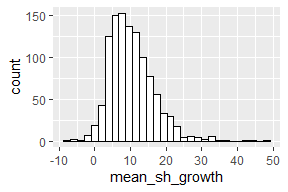
\includegraphics{1_data_prep_analyses_files/figure-latex/unnamed-chunk-12-1.pdf}

\begin{Shaded}
\begin{Highlighting}[]
\FunctionTok{plot}\NormalTok{(}\FunctionTok{ggpredict}\NormalTok{(model\_offpsring\_LFD,}\AttributeTok{terms=}\FunctionTok{c}\NormalTok{(}\StringTok{"treat"}\NormalTok{)))}
\end{Highlighting}
\end{Shaded}

\includegraphics{1_data_prep_analyses_files/figure-latex/unnamed-chunk-12-2.pdf}

\begin{Shaded}
\begin{Highlighting}[]
\FunctionTok{plot}\NormalTok{(}\FunctionTok{ggpredict}\NormalTok{(model\_offpsring\_date50,}\AttributeTok{terms=}\FunctionTok{c}\NormalTok{(}\StringTok{"treat"}\NormalTok{)))}
\end{Highlighting}
\end{Shaded}

\includegraphics{1_data_prep_analyses_files/figure-latex/unnamed-chunk-12-3.pdf}

\begin{Shaded}
\begin{Highlighting}[]
\FunctionTok{plot}\NormalTok{(}\FunctionTok{ggpredict}\NormalTok{(model\_offpsring\_date50,}\AttributeTok{terms=}\FunctionTok{c}\NormalTok{(}\StringTok{"temp\_father"}\NormalTok{)))}
\end{Highlighting}
\end{Shaded}

\includegraphics{1_data_prep_analyses_files/figure-latex/unnamed-chunk-12-4.pdf}

Plot predictions of interactions (NS)

\begin{Shaded}
\begin{Highlighting}[]
\FunctionTok{plot}\NormalTok{(}\FunctionTok{ggpredict}\NormalTok{(model\_offpsring\_FFD,}\AttributeTok{terms=}\FunctionTok{c}\NormalTok{(}\StringTok{"temp\_mother"}\NormalTok{,}\StringTok{"treat"}\NormalTok{)))}
\end{Highlighting}
\end{Shaded}

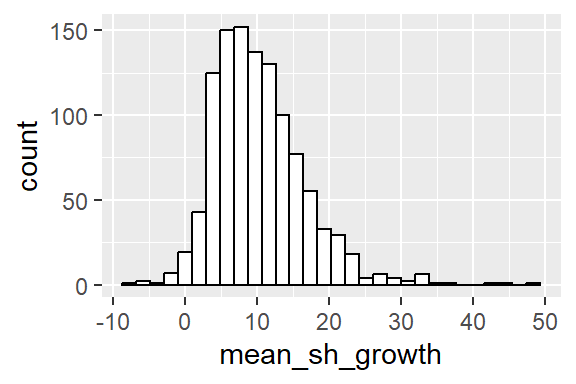
\includegraphics{1_data_prep_analyses_files/figure-latex/unnamed-chunk-13-1.pdf}

\begin{Shaded}
\begin{Highlighting}[]
\FunctionTok{plot}\NormalTok{(}\FunctionTok{ggpredict}\NormalTok{(model\_offpsring\_LFD,}\AttributeTok{terms=}\FunctionTok{c}\NormalTok{(}\StringTok{"temp\_mother"}\NormalTok{,}\StringTok{"treat"}\NormalTok{)))}
\end{Highlighting}
\end{Shaded}

\includegraphics{1_data_prep_analyses_files/figure-latex/unnamed-chunk-13-2.pdf}

\begin{Shaded}
\begin{Highlighting}[]
\FunctionTok{plot}\NormalTok{(}\FunctionTok{ggpredict}\NormalTok{(model\_offpsring\_date50,}\AttributeTok{terms=}\FunctionTok{c}\NormalTok{(}\StringTok{"temp\_mother"}\NormalTok{,}\StringTok{"treat"}\NormalTok{)))}
\end{Highlighting}
\end{Shaded}

\includegraphics{1_data_prep_analyses_files/figure-latex/unnamed-chunk-13-3.pdf}

\begin{Shaded}
\begin{Highlighting}[]
\FunctionTok{plot}\NormalTok{(}\FunctionTok{ggpredict}\NormalTok{(model\_offpsring\_FFD,}\AttributeTok{terms=}\FunctionTok{c}\NormalTok{(}\StringTok{"temp\_father"}\NormalTok{,}\StringTok{"treat"}\NormalTok{)))}
\end{Highlighting}
\end{Shaded}

\includegraphics{1_data_prep_analyses_files/figure-latex/unnamed-chunk-13-4.pdf}

\begin{Shaded}
\begin{Highlighting}[]
\FunctionTok{plot}\NormalTok{(}\FunctionTok{ggpredict}\NormalTok{(model\_offpsring\_LFD,}\AttributeTok{terms=}\FunctionTok{c}\NormalTok{(}\StringTok{"temp\_father"}\NormalTok{,}\StringTok{"treat"}\NormalTok{)))}
\end{Highlighting}
\end{Shaded}

\includegraphics{1_data_prep_analyses_files/figure-latex/unnamed-chunk-13-5.pdf}

\begin{Shaded}
\begin{Highlighting}[]
\FunctionTok{plot}\NormalTok{(}\FunctionTok{ggpredict}\NormalTok{(model\_offpsring\_date50,}\AttributeTok{terms=}\FunctionTok{c}\NormalTok{(}\StringTok{"temp\_father"}\NormalTok{,}\StringTok{"treat"}\NormalTok{)))}
\end{Highlighting}
\end{Shaded}

\includegraphics{1_data_prep_analyses_files/figure-latex/unnamed-chunk-13-6.pdf}

\hypertarget{with-parents}{%
\subsection{With parents}\label{with-parents}}

\begin{Shaded}
\begin{Highlighting}[]
\NormalTok{model\_parents\_FFD}\OtherTok{\textless{}{-}}\FunctionTok{lm}\NormalTok{(FFD}\SpecialCharTok{\textasciitilde{}}\NormalTok{temp}\SpecialCharTok{*}\NormalTok{treat,data\_parents)}
\NormalTok{model\_parents\_LFD}\OtherTok{\textless{}{-}}\FunctionTok{lm}\NormalTok{(LFD}\SpecialCharTok{\textasciitilde{}}\NormalTok{temp}\SpecialCharTok{*}\NormalTok{treat,data\_parents)}
\NormalTok{model\_parents\_date50}\OtherTok{\textless{}{-}}\FunctionTok{lm}\NormalTok{(date50}\SpecialCharTok{\textasciitilde{}}\NormalTok{temp}\SpecialCharTok{*}\NormalTok{treat,data\_parents)}
\end{Highlighting}
\end{Shaded}

\begin{Shaded}
\begin{Highlighting}[]
\FunctionTok{kable}\NormalTok{(}\FunctionTok{tidy}\NormalTok{(model\_parents\_FFD),}\AttributeTok{digits=}\FunctionTok{c}\NormalTok{(}\DecValTok{3}\NormalTok{,}\DecValTok{3}\NormalTok{,}\DecValTok{2}\NormalTok{,}\DecValTok{3}\NormalTok{))}
\end{Highlighting}
\end{Shaded}

\begin{longtable}[]{@{}lrrrr@{}}
\toprule()
term & estimate & std.error & statistic & p.value \\
\midrule()
\endhead
(Intercept) & 121.361 & 1.78 & 68.309 & 0.000 \\
temp & 0.031 & 0.08 & 0.388 & 0.698 \\
treatunheated & 4.295 & 2.50 & 1.719 & 0.087 \\
temp:treatunheated & 0.077 & 0.11 & 0.704 & 0.482 \\
\bottomrule()
\end{longtable}

\begin{Shaded}
\begin{Highlighting}[]
\FunctionTok{kable}\NormalTok{(}\FunctionTok{tidy}\NormalTok{(model\_parents\_LFD),}\AttributeTok{digits=}\FunctionTok{c}\NormalTok{(}\DecValTok{3}\NormalTok{,}\DecValTok{3}\NormalTok{,}\DecValTok{2}\NormalTok{,}\DecValTok{3}\NormalTok{))}
\end{Highlighting}
\end{Shaded}

\begin{longtable}[]{@{}lrrrr@{}}
\toprule()
term & estimate & std.error & statistic & p.value \\
\midrule()
\endhead
(Intercept) & 133.919 & 1.78 & 75.383 & 0.000 \\
temp & 0.146 & 0.08 & 1.837 & 0.068 \\
treatunheated & 6.150 & 2.48 & 2.477 & 0.014 \\
temp:treatunheated & 0.075 & 0.11 & 0.693 & 0.489 \\
\bottomrule()
\end{longtable}

\begin{Shaded}
\begin{Highlighting}[]
\FunctionTok{kable}\NormalTok{(}\FunctionTok{tidy}\NormalTok{(model\_parents\_date50),}\AttributeTok{digits=}\FunctionTok{c}\NormalTok{(}\DecValTok{3}\NormalTok{,}\DecValTok{3}\NormalTok{,}\DecValTok{2}\NormalTok{,}\DecValTok{3}\NormalTok{))}
\end{Highlighting}
\end{Shaded}

\begin{longtable}[]{@{}lrrrr@{}}
\toprule()
term & estimate & std.error & statistic & p.value \\
\midrule()
\endhead
(Intercept) & 124.469 & 1.37 & 90.620 & 0.000 \\
temp & 0.140 & 0.06 & 2.274 & 0.024 \\
treatunheated & 6.072 & 1.93 & 3.143 & 0.002 \\
temp:treatunheated & -0.009 & 0.08 & -0.105 & 0.917 \\
\bottomrule()
\end{longtable}

Save models as HTML table

\begin{Shaded}
\begin{Highlighting}[]
\FunctionTok{tab\_model}\NormalTok{(model\_parents\_FFD,model\_parents\_LFD,model\_parents\_date50,}
          \AttributeTok{transform=}\ConstantTok{NULL}\NormalTok{,}\AttributeTok{show.ci=}\NormalTok{F,}\AttributeTok{show.se=}\NormalTok{T,}\AttributeTok{show.stat=}\NormalTok{T,}\AttributeTok{digits=}\DecValTok{3}\NormalTok{,}
          \AttributeTok{dv.labels=}\FunctionTok{c}\NormalTok{(}\StringTok{"FFD"}\NormalTok{,}\StringTok{"LFD"}\NormalTok{,}\StringTok{"date50"}\NormalTok{),}
          \AttributeTok{file=}\StringTok{"output/tables/Table\_models\_parents.html"}\NormalTok{,}
          \AttributeTok{title=}\StringTok{"Models parents"}\NormalTok{)}
\end{Highlighting}
\end{Shaded}

Models parents

~

FFD

LFD

date50

Predictors

Estimates

std. Error

Statistic

p

Estimates

std. Error

Statistic

p

Estimates

std. Error

Statistic

p

(Intercept)

121.361

1.777

68.309

\textless0.001

133.919

1.777

75.383

\textless0.001

124.469

1.374

90.620

\textless0.001

temp

0.031

0.080

0.388

0.698

0.146

0.079

1.837

0.068

0.140

0.062

2.274

0.024

treat {[}unheated{]}

4.295

2.499

1.719

0.087

6.150

2.483

2.477

0.014

6.072

1.932

3.143

0.002

temp × treat {[}unheated{]}

0.077

0.109

0.704

0.482

0.075

0.108

0.693

0.489

-0.009

0.084

-0.105

0.917

Observations

186

185

186

R2 / R2 adjusted

0.129 / 0.114

0.239 / 0.226

0.228 / 0.215

Only effect of treatment is significant for LFD (not for FFD, p=0.087,
signif when using Anova - type II AOV), also temp for date 50 (p=0.068
for temp in the model for LFD).

Plot predictions of significant effects

\begin{Shaded}
\begin{Highlighting}[]
\FunctionTok{plot}\NormalTok{(}\FunctionTok{ggpredict}\NormalTok{(model\_parents\_FFD,}\AttributeTok{terms=}\FunctionTok{c}\NormalTok{(}\StringTok{"treat"}\NormalTok{)))}
\end{Highlighting}
\end{Shaded}

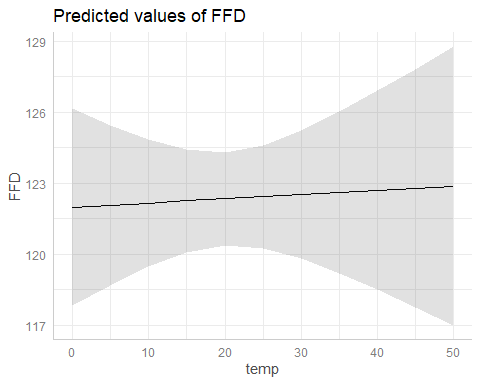
\includegraphics{1_data_prep_analyses_files/figure-latex/unnamed-chunk-17-1.pdf}

\begin{Shaded}
\begin{Highlighting}[]
\FunctionTok{plot}\NormalTok{(}\FunctionTok{ggpredict}\NormalTok{(model\_parents\_LFD,}\AttributeTok{terms=}\FunctionTok{c}\NormalTok{(}\StringTok{"treat"}\NormalTok{)))}
\end{Highlighting}
\end{Shaded}

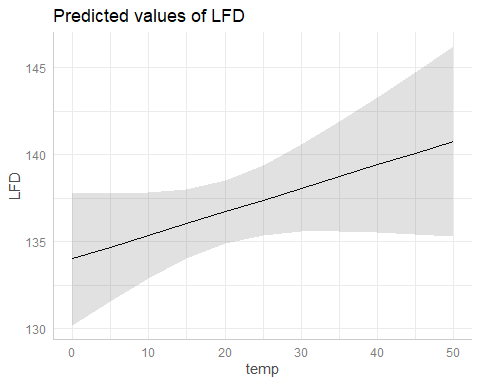
\includegraphics{1_data_prep_analyses_files/figure-latex/unnamed-chunk-17-2.pdf}

\begin{Shaded}
\begin{Highlighting}[]
\FunctionTok{plot}\NormalTok{(}\FunctionTok{ggpredict}\NormalTok{(model\_parents\_date50,}\AttributeTok{terms=}\FunctionTok{c}\NormalTok{(}\StringTok{"treat"}\NormalTok{)))}
\end{Highlighting}
\end{Shaded}

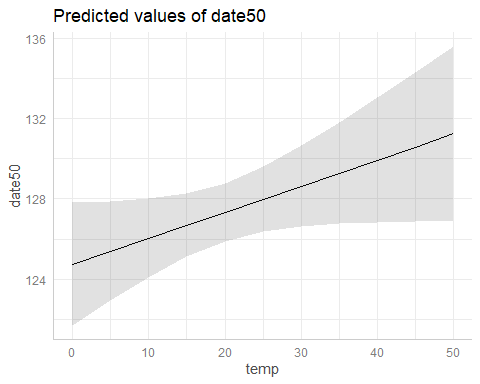
\includegraphics{1_data_prep_analyses_files/figure-latex/unnamed-chunk-17-3.pdf}

\begin{Shaded}
\begin{Highlighting}[]
\FunctionTok{plot}\NormalTok{(}\FunctionTok{ggpredict}\NormalTok{(model\_parents\_date50,}\AttributeTok{terms=}\FunctionTok{c}\NormalTok{(}\StringTok{"temp"}\NormalTok{)))}
\end{Highlighting}
\end{Shaded}

\includegraphics{1_data_prep_analyses_files/figure-latex/unnamed-chunk-17-4.pdf}

Plot predictions of interactions (NS)

\begin{Shaded}
\begin{Highlighting}[]
\FunctionTok{plot}\NormalTok{(}\FunctionTok{ggpredict}\NormalTok{(model\_parents\_FFD,}\AttributeTok{terms=}\FunctionTok{c}\NormalTok{(}\StringTok{"temp"}\NormalTok{,}\StringTok{"treat"}\NormalTok{)))}
\end{Highlighting}
\end{Shaded}

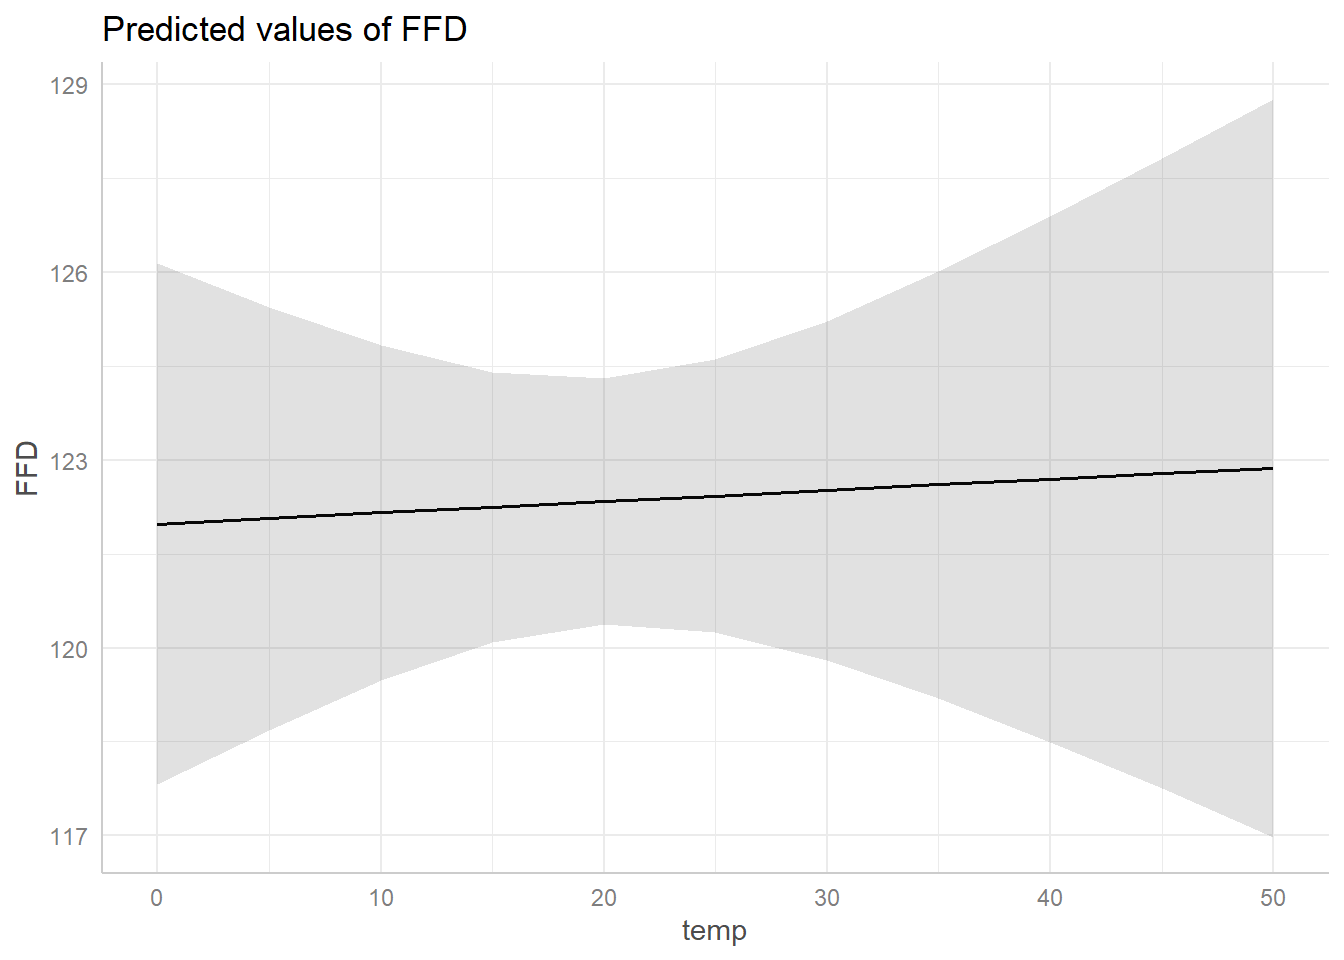
\includegraphics{1_data_prep_analyses_files/figure-latex/unnamed-chunk-18-1.pdf}

\begin{Shaded}
\begin{Highlighting}[]
\FunctionTok{plot}\NormalTok{(}\FunctionTok{ggpredict}\NormalTok{(model\_parents\_LFD,}\AttributeTok{terms=}\FunctionTok{c}\NormalTok{(}\StringTok{"temp"}\NormalTok{,}\StringTok{"treat"}\NormalTok{)))}
\end{Highlighting}
\end{Shaded}

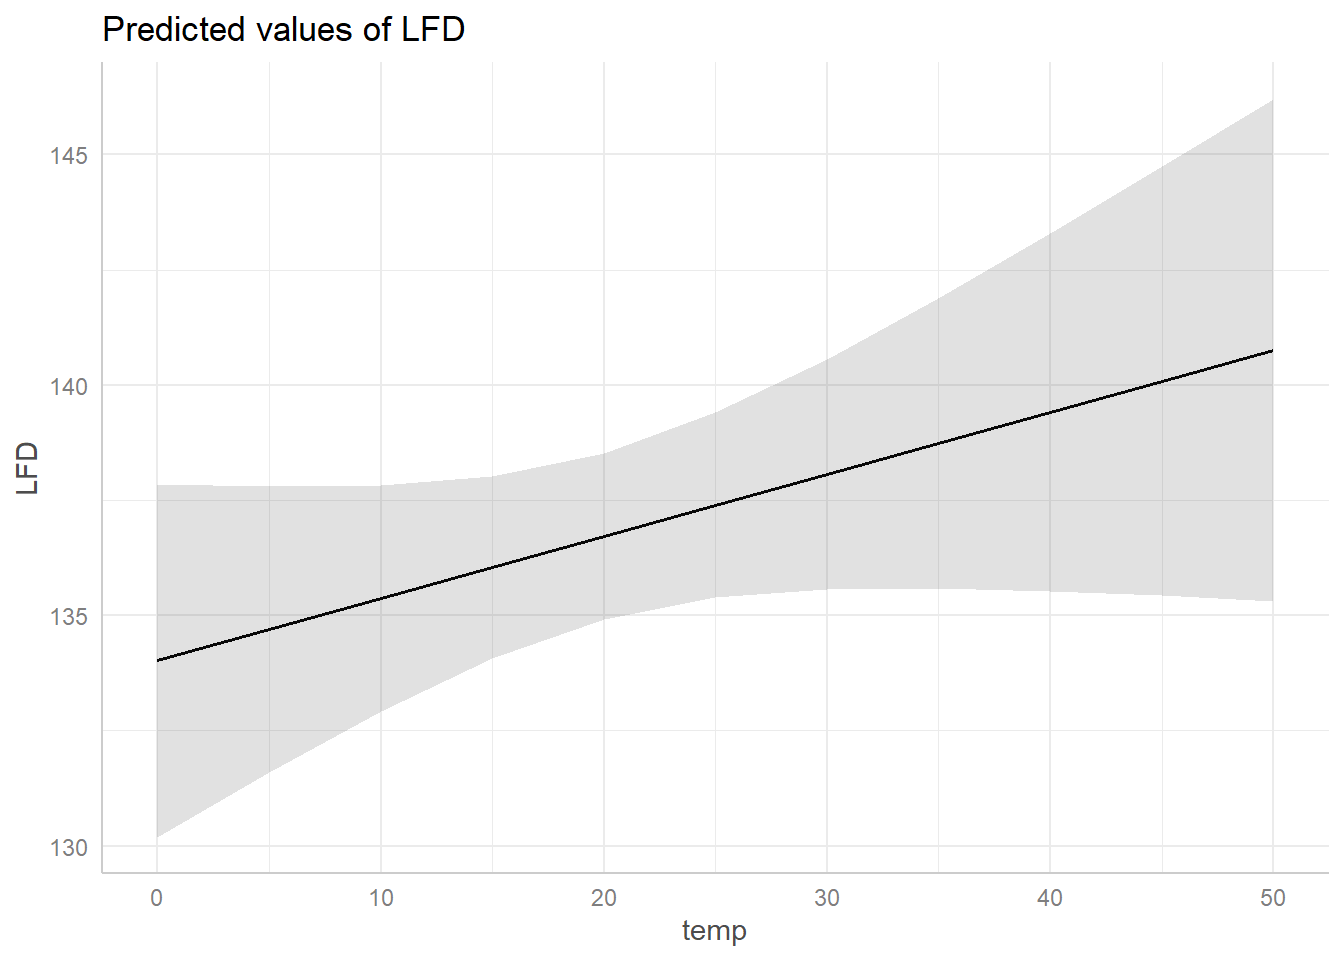
\includegraphics{1_data_prep_analyses_files/figure-latex/unnamed-chunk-18-2.pdf}

\begin{Shaded}
\begin{Highlighting}[]
\FunctionTok{plot}\NormalTok{(}\FunctionTok{ggpredict}\NormalTok{(model\_parents\_date50,}\AttributeTok{terms=}\FunctionTok{c}\NormalTok{(}\StringTok{"temp"}\NormalTok{,}\StringTok{"treat"}\NormalTok{)))}
\end{Highlighting}
\end{Shaded}

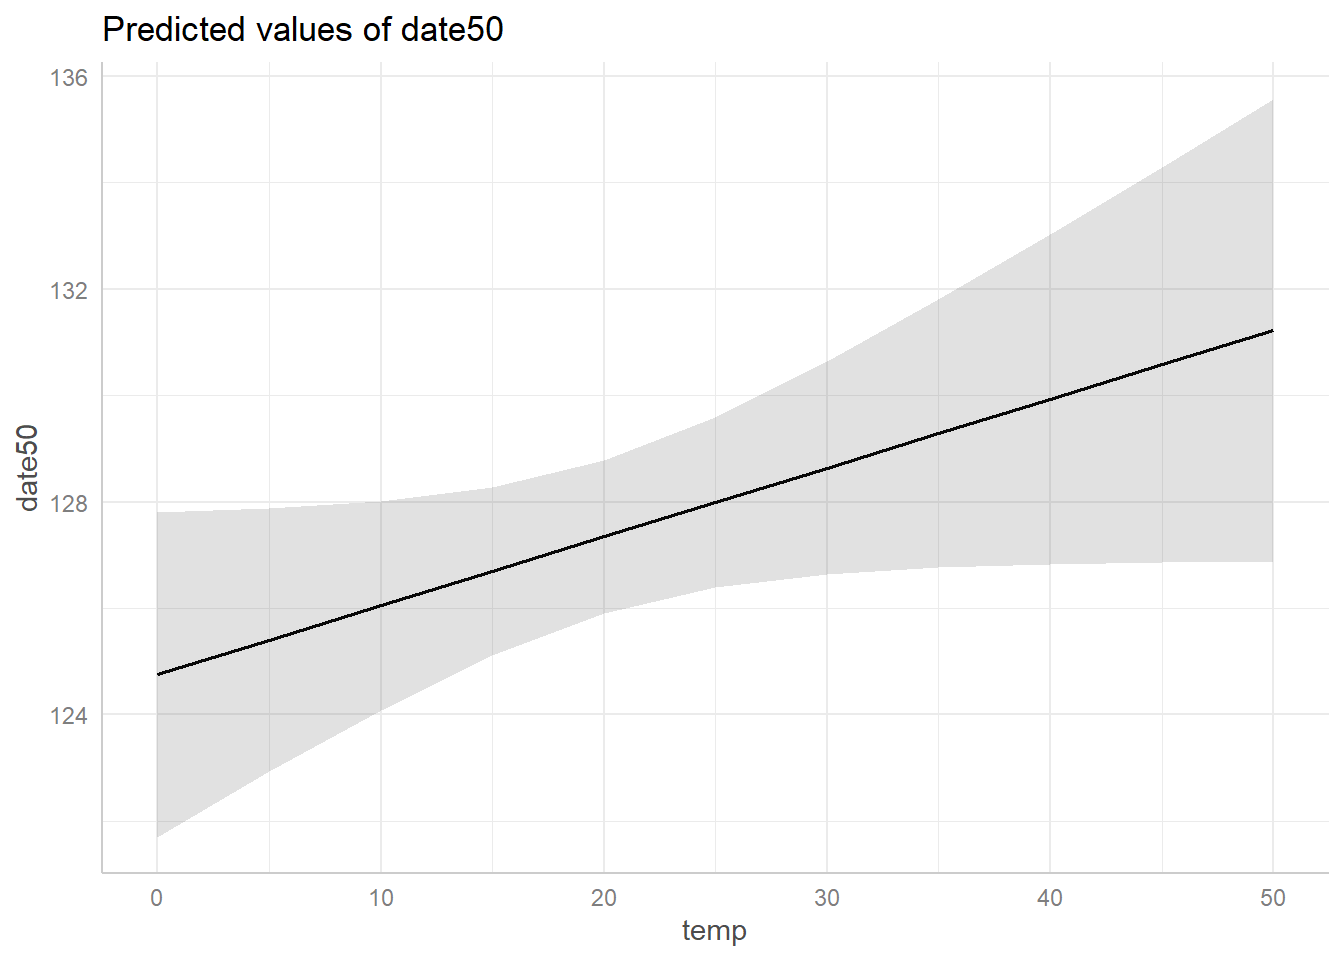
\includegraphics{1_data_prep_analyses_files/figure-latex/unnamed-chunk-18-3.pdf}

\hypertarget{heritability}{%
\subsection{Heritability}\label{heritability}}

Construct models

\begin{Shaded}
\begin{Highlighting}[]
\NormalTok{model\_her\_FFD}\OtherTok{\textless{}{-}}\FunctionTok{lmer}\NormalTok{(FFD}\SpecialCharTok{\textasciitilde{}}\NormalTok{(}\DecValTok{1}\SpecialCharTok{|}\NormalTok{father)}\SpecialCharTok{+}\NormalTok{(}\DecValTok{1}\SpecialCharTok{|}\NormalTok{mother),data\_exp,}\AttributeTok{REML=}\NormalTok{T)}
\NormalTok{model\_her\_LFD}\OtherTok{\textless{}{-}}\FunctionTok{lmer}\NormalTok{(LFD}\SpecialCharTok{\textasciitilde{}}\NormalTok{(}\DecValTok{1}\SpecialCharTok{|}\NormalTok{father)}\SpecialCharTok{+}\NormalTok{(}\DecValTok{1}\SpecialCharTok{|}\NormalTok{mother),data\_exp,}\AttributeTok{REML=}\NormalTok{T)}
\NormalTok{model\_her\_date50}\OtherTok{\textless{}{-}}\FunctionTok{lmer}\NormalTok{(date50}\SpecialCharTok{\textasciitilde{}}\NormalTok{(}\DecValTok{1}\SpecialCharTok{|}\NormalTok{father)}\SpecialCharTok{+}\NormalTok{(}\DecValTok{1}\SpecialCharTok{|}\NormalTok{mother),data\_exp,}\AttributeTok{REML=}\NormalTok{T)}
\FunctionTok{summary}\NormalTok{(model\_her\_FFD)}
\end{Highlighting}
\end{Shaded}

\begin{verbatim}
## Linear mixed model fit by REML ['lmerMod']
## Formula: FFD ~ (1 | father) + (1 | mother)
##    Data: data_exp
## 
## REML criterion at convergence: 6068.1
## 
## Scaled residuals: 
##     Min      1Q  Median      3Q     Max 
## -2.6485 -0.6912  0.0054  0.5641  4.2413 
## 
## Random effects:
##  Groups   Name        Variance Std.Dev.
##  mother   (Intercept) 11.360   3.370   
##  father   (Intercept)  3.515   1.875   
##  Residual             72.134   8.493   
## Number of obs: 844, groups:  mother, 25; father, 24
## 
## Fixed effects:
##             Estimate Std. Error t value
## (Intercept) 124.8684     0.8353   149.5
\end{verbatim}

\begin{Shaded}
\begin{Highlighting}[]
\FunctionTok{summary}\NormalTok{(model\_her\_LFD)}
\end{Highlighting}
\end{Shaded}

\begin{verbatim}
## Linear mixed model fit by REML ['lmerMod']
## Formula: LFD ~ (1 | father) + (1 | mother)
##    Data: data_exp
## 
## REML criterion at convergence: 6395.7
## 
## Scaled residuals: 
##      Min       1Q   Median       3Q      Max 
## -2.69822 -0.77948 -0.06719  0.74271  2.39390 
## 
## Random effects:
##  Groups   Name        Variance Std.Dev.
##  mother   (Intercept)   6.289   2.508  
##  father   (Intercept)   2.090   1.446  
##  Residual             108.817  10.432  
## Number of obs: 845, groups:  mother, 25; father, 24
## 
## Fixed effects:
##             Estimate Std. Error t value
## (Intercept) 143.7550     0.6912     208
\end{verbatim}

\begin{Shaded}
\begin{Highlighting}[]
\FunctionTok{summary}\NormalTok{(model\_her\_date50)}
\end{Highlighting}
\end{Shaded}

\begin{verbatim}
## Linear mixed model fit by REML ['lmerMod']
## Formula: date50 ~ (1 | father) + (1 | mother)
##    Data: data_exp
## 
## REML criterion at convergence: 5885.2
## 
## Scaled residuals: 
##     Min      1Q  Median      3Q     Max 
## -2.4068 -0.7115  0.0081  0.5983  3.8863 
## 
## Random effects:
##  Groups   Name        Variance Std.Dev.
##  mother   (Intercept)  8.694   2.949   
##  father   (Intercept)  1.680   1.296   
##  Residual             58.046   7.619   
## Number of obs: 845, groups:  mother, 25; father, 24
## 
## Fixed effects:
##             Estimate Std. Error t value
## (Intercept) 131.4959     0.7036   186.9
\end{verbatim}

Likelihood ratio test

\begin{Shaded}
\begin{Highlighting}[]
\NormalTok{model\_her\_FFD\_LR}\OtherTok{\textless{}{-}}\FunctionTok{lmer}\NormalTok{(FFD}\SpecialCharTok{\textasciitilde{}}\NormalTok{(}\DecValTok{1}\SpecialCharTok{|}\NormalTok{father)}\SpecialCharTok{+}\NormalTok{(}\DecValTok{1}\SpecialCharTok{|}\NormalTok{mother),data\_exp,}\AttributeTok{REML=}\NormalTok{F)}
\NormalTok{model\_her\_LFD\_LR}\OtherTok{\textless{}{-}}\FunctionTok{lmer}\NormalTok{(LFD}\SpecialCharTok{\textasciitilde{}}\NormalTok{(}\DecValTok{1}\SpecialCharTok{|}\NormalTok{father)}\SpecialCharTok{+}\NormalTok{(}\DecValTok{1}\SpecialCharTok{|}\NormalTok{mother),data\_exp,}\AttributeTok{REML=}\NormalTok{F)}
\NormalTok{model\_her\_date50\_LR}\OtherTok{\textless{}{-}}\FunctionTok{lmer}\NormalTok{(date50}\SpecialCharTok{\textasciitilde{}}\NormalTok{(}\DecValTok{1}\SpecialCharTok{|}\NormalTok{father)}\SpecialCharTok{+}\NormalTok{(}\DecValTok{1}\SpecialCharTok{|}\NormalTok{mother),data\_exp,}\AttributeTok{REML=}\NormalTok{F)}
\CommentTok{\# REML=FALSE because we want to compare models on likelihood  }

\CommentTok{\# model without random (father)}
\NormalTok{model\_her\_FFD\_LR\_mother}\OtherTok{\textless{}{-}}\FunctionTok{lmer}\NormalTok{(FFD}\SpecialCharTok{\textasciitilde{}}\NormalTok{(}\DecValTok{1}\SpecialCharTok{|}\NormalTok{mother),data\_exp,}\AttributeTok{REML=}\NormalTok{F)}
\NormalTok{model\_her\_LFD\_LR\_mother}\OtherTok{\textless{}{-}}\FunctionTok{lmer}\NormalTok{(LFD}\SpecialCharTok{\textasciitilde{}}\NormalTok{(}\DecValTok{1}\SpecialCharTok{|}\NormalTok{mother),data\_exp,}\AttributeTok{REML=}\NormalTok{F)}
\NormalTok{model\_her\_date50\_LR\_mother}\OtherTok{\textless{}{-}}\FunctionTok{lmer}\NormalTok{(date50}\SpecialCharTok{\textasciitilde{}}\NormalTok{(}\DecValTok{1}\SpecialCharTok{|}\NormalTok{mother),data\_exp,}\AttributeTok{REML=}\NormalTok{F)}

\CommentTok{\# model without random (mother)}
\NormalTok{model\_her\_FFD\_LR\_father}\OtherTok{\textless{}{-}}\FunctionTok{lmer}\NormalTok{(FFD}\SpecialCharTok{\textasciitilde{}}\NormalTok{(}\DecValTok{1}\SpecialCharTok{|}\NormalTok{father),data\_exp,}\AttributeTok{REML=}\NormalTok{F)}
\NormalTok{model\_her\_LFD\_LR\_father}\OtherTok{\textless{}{-}}\FunctionTok{lmer}\NormalTok{(LFD}\SpecialCharTok{\textasciitilde{}}\NormalTok{(}\DecValTok{1}\SpecialCharTok{|}\NormalTok{father),data\_exp,}\AttributeTok{REML=}\NormalTok{F)}
\NormalTok{model\_her\_date50\_LR\_father}\OtherTok{\textless{}{-}}\FunctionTok{lmer}\NormalTok{(date50}\SpecialCharTok{\textasciitilde{}}\NormalTok{(}\DecValTok{1}\SpecialCharTok{|}\NormalTok{father),data\_exp,}\AttributeTok{REML=}\NormalTok{F)}

\CommentTok{\# Father effect? Yes, in FFD and date50}
\FunctionTok{anova}\NormalTok{(model\_her\_FFD\_LR\_mother, model\_her\_FFD\_LR)}
\end{Highlighting}
\end{Shaded}

\begin{verbatim}
## Data: data_exp
## Models:
## model_her_FFD_LR_mother: FFD ~ (1 | mother)
## model_her_FFD_LR: FFD ~ (1 | father) + (1 | mother)
##                         npar    AIC    BIC  logLik deviance  Chisq Df
## model_her_FFD_LR_mother    3 6086.2 6100.4 -3040.1   6080.2          
## model_her_FFD_LR           4 6077.6 6096.5 -3034.8   6069.6 10.652  1
##                         Pr(>Chisq)   
## model_her_FFD_LR_mother              
## model_her_FFD_LR            0.0011 **
## ---
## Signif. codes:  0 '***' 0.001 '**' 0.01 '*' 0.05 '.' 0.1 ' ' 1
\end{verbatim}

\begin{Shaded}
\begin{Highlighting}[]
\FunctionTok{anova}\NormalTok{(model\_her\_LFD\_LR\_mother, model\_her\_LFD\_LR)}
\end{Highlighting}
\end{Shaded}

\begin{verbatim}
## Data: data_exp
## Models:
## model_her_LFD_LR_mother: LFD ~ (1 | mother)
## model_her_LFD_LR: LFD ~ (1 | father) + (1 | mother)
##                         npar    AIC    BIC  logLik deviance  Chisq Df
## model_her_LFD_LR_mother    3 6405.3 6419.5 -3199.7   6399.3          
## model_her_LFD_LR           4 6404.7 6423.7 -3198.4   6396.7 2.5734  1
##                         Pr(>Chisq)
## model_her_LFD_LR_mother           
## model_her_LFD_LR            0.1087
\end{verbatim}

\begin{Shaded}
\begin{Highlighting}[]
\FunctionTok{anova}\NormalTok{(model\_her\_date50\_LR\_mother, model\_her\_date50\_LR)}
\end{Highlighting}
\end{Shaded}

\begin{verbatim}
## Data: data_exp
## Models:
## model_her_date50_LR_mother: date50 ~ (1 | mother)
## model_her_date50_LR: date50 ~ (1 | father) + (1 | mother)
##                            npar    AIC    BIC  logLik deviance Chisq Df
## model_her_date50_LR_mother    3 5897.7 5911.9 -2945.8   5891.7         
## model_her_date50_LR           4 5894.3 5913.3 -2943.2   5886.3 5.379  1
##                            Pr(>Chisq)  
## model_her_date50_LR_mother             
## model_her_date50_LR           0.02038 *
## ---
## Signif. codes:  0 '***' 0.001 '**' 0.01 '*' 0.05 '.' 0.1 ' ' 1
\end{verbatim}

\begin{Shaded}
\begin{Highlighting}[]
\CommentTok{\# Mother effect? Yes, in FFD, LFD and date50}
\FunctionTok{anova}\NormalTok{(model\_her\_FFD\_LR\_father, model\_her\_FFD\_LR)}
\end{Highlighting}
\end{Shaded}

\begin{verbatim}
## Data: data_exp
## Models:
## model_her_FFD_LR_father: FFD ~ (1 | father)
## model_her_FFD_LR: FFD ~ (1 | father) + (1 | mother)
##                         npar    AIC    BIC  logLik deviance  Chisq Df
## model_her_FFD_LR_father    3 6135.7 6149.9 -3064.8   6129.7          
## model_her_FFD_LR           4 6077.6 6096.5 -3034.8   6069.6 60.128  1
##                         Pr(>Chisq)    
## model_her_FFD_LR_father               
## model_her_FFD_LR          8.89e-15 ***
## ---
## Signif. codes:  0 '***' 0.001 '**' 0.01 '*' 0.05 '.' 0.1 ' ' 1
\end{verbatim}

\begin{Shaded}
\begin{Highlighting}[]
\FunctionTok{anova}\NormalTok{(model\_her\_LFD\_LR\_father, model\_her\_LFD\_LR)}
\end{Highlighting}
\end{Shaded}

\begin{verbatim}
## Data: data_exp
## Models:
## model_her_LFD_LR_father: LFD ~ (1 | father)
## model_her_LFD_LR: LFD ~ (1 | father) + (1 | mother)
##                         npar    AIC    BIC  logLik deviance  Chisq Df
## model_her_LFD_LR_father    3 6416.5 6430.7 -3205.2   6410.5          
## model_her_LFD_LR           4 6404.7 6423.7 -3198.4   6396.7 13.706  1
##                         Pr(>Chisq)    
## model_her_LFD_LR_father               
## model_her_LFD_LR         0.0002138 ***
## ---
## Signif. codes:  0 '***' 0.001 '**' 0.01 '*' 0.05 '.' 0.1 ' ' 1
\end{verbatim}

\begin{Shaded}
\begin{Highlighting}[]
\FunctionTok{anova}\NormalTok{(model\_her\_date50\_LR\_father, model\_her\_date50\_LR)}
\end{Highlighting}
\end{Shaded}

\begin{verbatim}
## Data: data_exp
## Models:
## model_her_date50_LR_father: date50 ~ (1 | father)
## model_her_date50_LR: date50 ~ (1 | father) + (1 | mother)
##                            npar    AIC    BIC  logLik deviance  Chisq Df
## model_her_date50_LR_father    3 5944.3 5958.5 -2969.2   5938.3          
## model_her_date50_LR           4 5894.3 5913.3 -2943.2   5886.3 51.996  1
##                            Pr(>Chisq)    
## model_her_date50_LR_father               
## model_her_date50_LR         5.561e-13 ***
## ---
## Signif. codes:  0 '***' 0.001 '**' 0.01 '*' 0.05 '.' 0.1 ' ' 1
\end{verbatim}

Variance components

\begin{Shaded}
\begin{Highlighting}[]
\CommentTok{\# extract variance components}
\NormalTok{Variance\_FFD }\OtherTok{\textless{}{-}} \FunctionTok{as.data.frame}\NormalTok{(}\FunctionTok{VarCorr}\NormalTok{(model\_her\_FFD))[,}\DecValTok{4}\NormalTok{] }
\NormalTok{Variance\_LFD }\OtherTok{\textless{}{-}} \FunctionTok{as.data.frame}\NormalTok{(}\FunctionTok{VarCorr}\NormalTok{(model\_her\_LFD))[,}\DecValTok{4}\NormalTok{] }
\NormalTok{Variance\_date50 }\OtherTok{\textless{}{-}} \FunctionTok{as.data.frame}\NormalTok{(}\FunctionTok{VarCorr}\NormalTok{(model\_her\_date50))[,}\DecValTok{4}\NormalTok{] }
\CommentTok{\# Intra{-}class correlation}
\NormalTok{PropVar\_FFD }\OtherTok{\textless{}{-}}\NormalTok{ Variance\_FFD}\SpecialCharTok{/}\FunctionTok{sum}\NormalTok{(Variance\_FFD) }
\NormalTok{PropVar\_LFD }\OtherTok{\textless{}{-}}\NormalTok{ Variance\_LFD}\SpecialCharTok{/}\FunctionTok{sum}\NormalTok{(Variance\_LFD) }
\NormalTok{PropVar\_date50 }\OtherTok{\textless{}{-}}\NormalTok{ Variance\_date50}\SpecialCharTok{/}\FunctionTok{sum}\NormalTok{(Variance\_date50) }
\CommentTok{\# Proportional variance}
\end{Highlighting}
\end{Shaded}

Heritability and maternal effects

\begin{Shaded}
\begin{Highlighting}[]
\CommentTok{\# h\^{}2 (paternal effects)}
\DecValTok{4}\SpecialCharTok{*}\NormalTok{PropVar\_FFD[}\DecValTok{2}\NormalTok{]}
\end{Highlighting}
\end{Shaded}

\begin{verbatim}
## [1] 0.1615978
\end{verbatim}

\begin{Shaded}
\begin{Highlighting}[]
\DecValTok{4}\SpecialCharTok{*}\NormalTok{PropVar\_LFD[}\DecValTok{2}\NormalTok{]}
\end{Highlighting}
\end{Shaded}

\begin{verbatim}
## [1] 0.07132973
\end{verbatim}

\begin{Shaded}
\begin{Highlighting}[]
\DecValTok{4}\SpecialCharTok{*}\NormalTok{PropVar\_date50[}\DecValTok{2}\NormalTok{]}
\end{Highlighting}
\end{Shaded}

\begin{verbatim}
## [1] 0.09822599
\end{verbatim}

\begin{Shaded}
\begin{Highlighting}[]
\CommentTok{\# Because the additive genetic variance, VA,}
\CommentTok{\# is expected to be four times the among pollen‐donor variance }
\CommentTok{\# (Falconer \& Mackay, 1996; Lynch \& Walsh, 1998)}
\end{Highlighting}
\end{Shaded}

\begin{Shaded}
\begin{Highlighting}[]
\CommentTok{\# maternal effects}

\CommentTok{\# Maternal {-} paternal}
\CommentTok{\# {-}{-}{-}{-}{-}{-}{-}{-}{-}{-}{-}{-}{-}{-}{-}{-}{-}{-}{-}{-}{-}{-}}
\CommentTok{\# summed effects}

\NormalTok{(Variance\_FFD[}\DecValTok{1}\NormalTok{]}\SpecialCharTok{{-}}\NormalTok{Variance\_FFD[}\DecValTok{2}\NormalTok{])}\SpecialCharTok{/}\FunctionTok{sum}\NormalTok{(Variance\_FFD)}
\end{Highlighting}
\end{Shaded}

\begin{verbatim}
## [1] 0.09016114
\end{verbatim}

\begin{Shaded}
\begin{Highlighting}[]
\NormalTok{(Variance\_LFD[}\DecValTok{1}\NormalTok{]}\SpecialCharTok{{-}}\NormalTok{Variance\_LFD[}\DecValTok{2}\NormalTok{])}\SpecialCharTok{/}\FunctionTok{sum}\NormalTok{(Variance\_LFD)}
\end{Highlighting}
\end{Shaded}

\begin{verbatim}
## [1] 0.03582914
\end{verbatim}

\begin{Shaded}
\begin{Highlighting}[]
\NormalTok{(Variance\_date50[}\DecValTok{1}\NormalTok{]}\SpecialCharTok{{-}}\NormalTok{Variance\_date50[}\DecValTok{2}\NormalTok{])}\SpecialCharTok{/}\FunctionTok{sum}\NormalTok{(Variance\_date50)}
\end{Highlighting}
\end{Shaded}

\begin{verbatim}
## [1] 0.1025179
\end{verbatim}

Additive genetic effects explained 13.1 / 5.3 / 12.7 \% of the variation
in FFD / LFD / date50 among sibling plants (σ2 pollen donor = 3.5 / 2.1
/ 1,68, Likelihood ratio test, χ2 = 10.7 / 2.6 / 5.4, p = 0.001 / 0.109
/ 0,020). Maternal non‐genetic effects explained 4.0 / 1.8 / 2.5 \% of
the variation in FFD / LFD / date50 among sibling plants (σ2 pollen
recipient = 11.4 / 6.3 / 8.7, Likelihood ratio test, χ2 = 60.1 / 13.7 /
52.0, p \textless{} 0.001). The remaining 82.9 / 92.3 / 84.8 \% of the
variation in FFD / LFD / date50 was attributable to environmental
(residual) effects. h2? m2?

\hypertarget{mid-parent-value}{%
\section{Mid-parent value}\label{mid-parent-value}}

Merge data offspring and parents

\begin{Shaded}
\begin{Highlighting}[]
\NormalTok{data\_all}\OtherTok{\textless{}{-}}\NormalTok{data\_exp}\SpecialCharTok{\%\textgreater{}\%}
  \FunctionTok{left\_join}\NormalTok{(data\_parents}\SpecialCharTok{\%\textgreater{}\%}
              \FunctionTok{mutate}\NormalTok{(}\AttributeTok{id\_parent=}\FunctionTok{as.factor}\NormalTok{(id\_parent))}\SpecialCharTok{\%\textgreater{}\%}
              \FunctionTok{select}\NormalTok{(id\_parent,treat,FFD,LFD,date50)}\SpecialCharTok{\%\textgreater{}\%}
              \FunctionTok{rename}\NormalTok{(}\AttributeTok{treat\_parent=}\NormalTok{treat,}\AttributeTok{FFD\_parent=}\NormalTok{FFD,}\AttributeTok{LFD\_parent=}\NormalTok{LFD,}
                     \AttributeTok{date50\_parent=}\NormalTok{date50),}
            \FunctionTok{join\_by}\NormalTok{(mother}\SpecialCharTok{==}\NormalTok{id\_parent))}
\end{Highlighting}
\end{Shaded}

Does not work so far because each row in x matches several rows in y.

\hypertarget{to-do}{%
\section{TO DO}\label{to-do}}

Include id of crossing (mother\_father) as random effect? See how to do
with mother and father (does not change much?) Run models with mean temp
of mother and father as part of results. Heritability of FT? Regress FT
of offspring on FT of parents. ``Biparental value'' (mean) or separately
fathers and mothers. And separately for each treatment. How much of the
FT of the offspring is explained by the FT of the parents. Check Elsa's
paper - code available to download - use!

\hypertarget{session-info}{%
\section{Session info}\label{session-info}}

\begin{Shaded}
\begin{Highlighting}[]
\FunctionTok{sessionInfo}\NormalTok{()}
\end{Highlighting}
\end{Shaded}

\begin{verbatim}
## R version 4.2.2 (2022-10-31 ucrt)
## Platform: x86_64-w64-mingw32/x64 (64-bit)
## Running under: Windows 10 x64 (build 19045)
## 
## Matrix products: default
## 
## locale:
## [1] LC_COLLATE=Swedish_Sweden.utf8  LC_CTYPE=Swedish_Sweden.utf8   
## [3] LC_MONETARY=Swedish_Sweden.utf8 LC_NUMERIC=C                   
## [5] LC_TIME=Swedish_Sweden.utf8    
## 
## attached base packages:
## [1] stats     graphics  grDevices utils     datasets  methods   base     
## 
## other attached packages:
##  [1] lme4_1.1-31         Matrix_1.5-1        knitr_1.42         
##  [4] broom.mixed_0.2.9.4 broom_1.0.3         jtools_2.2.1       
##  [7] sjPlot_2.8.12       car_3.1-1           carData_3.0-5      
## [10] glmmTMB_1.1.5       ggeffects_1.2.0     RColorBrewer_1.1-3 
## [13] readxl_1.4.2        lubridate_1.9.2     forcats_1.0.0      
## [16] stringr_1.5.0       dplyr_1.1.0         purrr_1.0.1        
## [19] readr_2.1.4         tidyr_1.3.0         tibble_3.1.8       
## [22] ggplot2_3.4.1       tidyverse_2.0.0    
## 
## loaded via a namespace (and not attached):
##  [1] nlme_3.1-160        insight_0.19.0      numDeriv_2016.8-1.1
##  [4] tools_4.2.2         TMB_1.9.2           backports_1.4.1    
##  [7] utf8_1.2.3          R6_2.5.1            sjlabelled_1.2.0   
## [10] colorspace_2.1-0    withr_2.5.0         tidyselect_1.2.0   
## [13] emmeans_1.8.4-1     compiler_4.2.2      performance_0.10.2 
## [16] cli_3.6.0           labeling_0.4.2      bayestestR_0.13.0  
## [19] scales_1.2.1        mvtnorm_1.1-3       digest_0.6.31      
## [22] minqa_1.2.5         rmarkdown_2.20      pkgconfig_2.0.3    
## [25] htmltools_0.5.4     parallelly_1.34.0   highr_0.10         
## [28] fastmap_1.1.1       rlang_1.0.6         rstudioapi_0.14    
## [31] generics_0.1.3      farver_2.1.1        magrittr_2.0.3     
## [34] parameters_0.20.2   Rcpp_1.0.10         munsell_0.5.0      
## [37] fansi_1.0.4         abind_1.4-5         lifecycle_1.0.3    
## [40] furrr_0.3.1         stringi_1.7.12      yaml_2.3.7         
## [43] MASS_7.3-58.1       grid_4.2.2          parallel_4.2.2     
## [46] listenv_0.9.0       sjmisc_2.8.9        crayon_1.5.2       
## [49] lattice_0.20-45     haven_2.5.2         splines_4.2.2      
## [52] pander_0.6.5        sjstats_0.18.2      hms_1.1.2          
## [55] pillar_1.8.1        boot_1.3-28         estimability_1.4.1 
## [58] effectsize_0.8.3    codetools_0.2-18    glue_1.6.2         
## [61] evaluate_0.20       modelr_0.1.10       vctrs_0.5.2        
## [64] nloptr_2.0.3        tzdb_0.3.0          cellranger_1.1.0   
## [67] gtable_0.3.1        future_1.32.0       datawizard_0.6.5   
## [70] xfun_0.37           xtable_1.8-4        coda_0.19-4        
## [73] timechange_0.2.0    globals_0.16.2      ellipsis_0.3.2
\end{verbatim}

\end{document}
